\documentclass[tikz,border=14pt]{standalone}
\usepackage[T1]{fontenc}
\usepackage[utf8]{inputenc}
\usepackage{helvet}
\renewcommand{\familydefault}{\sfdefault}
\usetikzlibrary{arrows.meta,positioning,calc,backgrounds,fit}

\definecolor{ich}{HTML}{D9602B}
\definecolor{ichhell}{HTML}{FBE9DF}
\definecolor{ki}{HTML}{2F5D8A}
\definecolor{kihell}{HTML}{E6EEF6}
\definecolor{ol}{HTML}{3C8D5A}
\definecolor{olhell}{HTML}{E4F2E9}
\definecolor{rr}{HTML}{6B4FA0}
\definecolor{rrhell}{HTML}{EEE9F6}
\definecolor{db}{HTML}{8A6A2E}
\definecolor{dbhell}{HTML}{F6F0E2}
\definecolor{grau}{HTML}{5A5F66}
\definecolor{bahn}{HTML}{F5F6F8}

\begin{document}
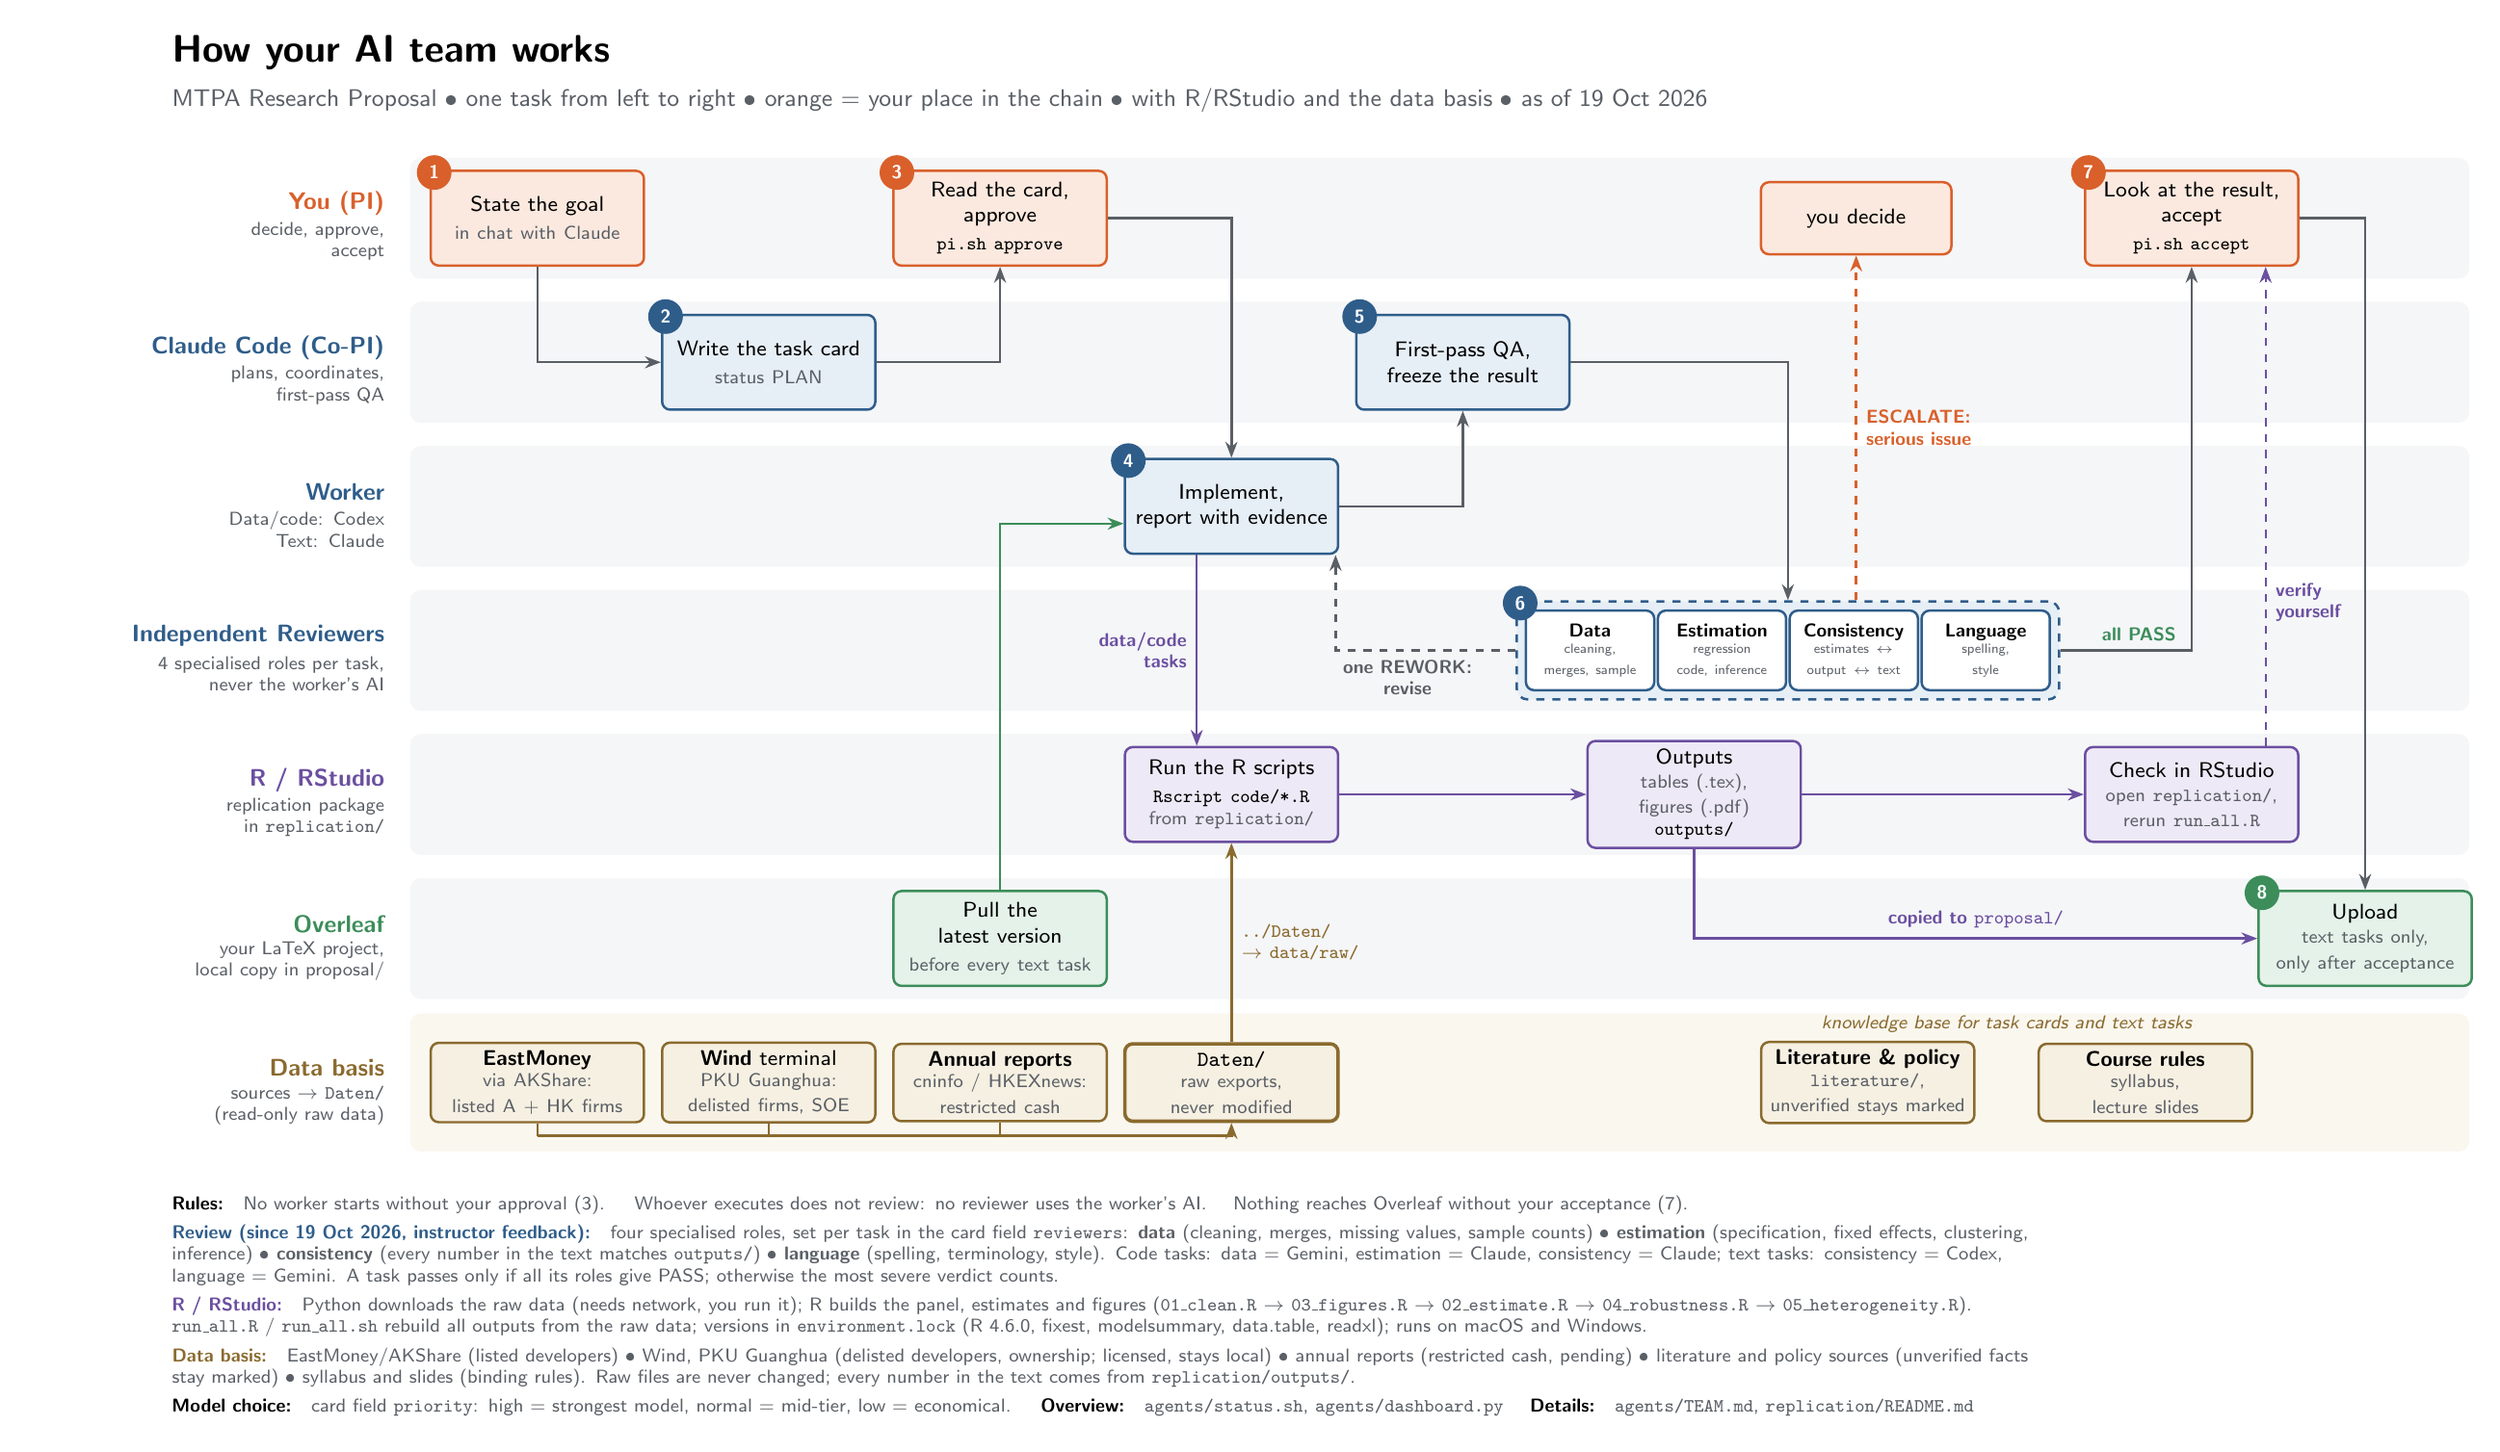
\begin{tikzpicture}[
  x=3.05cm, y=1.9cm,
  kasten/.style={rounded corners=3pt, draw=#1, line width=0.9pt, align=center,
                 text width=2.6cm, minimum height=1.25cm, font=\footnotesize, inner sep=3pt},
  ich/.style={kasten=ich, fill=ichhell},
  ki/.style={kasten=ki, fill=kihell},
  ol/.style={kasten=ol, fill=olhell},
  rr/.style={kasten=rr, fill=rrhell},
  db/.style={kasten=db, fill=dbhell, minimum height=1.0cm},
  rv/.style={kasten=ki, fill=white, text width=1.55cm, minimum height=1.05cm, font=\scriptsize, inner sep=2pt},
  pfeil/.style={-{Stealth[length=6pt]}, line width=0.9pt, draw=grau},
  lbl/.style={font=\scriptsize\bfseries, text=#1},
  nr/.style={circle, fill=#1, text=white, font=\scriptsize\bfseries, inner sep=1.3pt, minimum size=13pt},
  bahnname/.style={font=\small\bfseries, anchor=east, align=right, text width=4.6cm},
  bahnsub/.style={font=\scriptsize, text=grau, anchor=east, align=right, text width=4.6cm},
]

% ---------------------------------------------------------------- lanes
\begin{scope}[on background layer]
  \foreach \y in {6,5,4,3,2,1} {
    \fill[bahn, rounded corners=4pt] (0.45,\y-0.42) rectangle (9.35,\y+0.42);
  }
  \fill[dbhell!55, rounded corners=4pt] (0.45,-0.48) rectangle (9.35,0.48);
\end{scope}

\node[bahnname, text=ich] at (0.38,6.10) {You (PI)};
\node[bahnsub]            at (0.38,5.84) {decide, approve,\\accept};
\node[bahnname, text=ki]  at (0.38,5.10) {Claude Code (Co-PI)};
\node[bahnsub]            at (0.38,4.84) {plans, coordinates,\\first-pass QA};
\node[bahnname, text=ki]  at (0.38,4.10) {Worker};
\node[bahnsub]            at (0.38,3.84) {Data/code: Codex\\Text: Claude};
\node[bahnname, text=ki]  at (0.38,3.10) {Independent Reviewers};
\node[bahnsub]            at (0.38,2.84) {4 specialised roles per task,\\never the worker's AI};
\node[bahnname, text=rr]  at (0.38,2.10) {R / RStudio};
\node[bahnsub]            at (0.38,1.84) {replication package\\in \texttt{replication/}};
\node[bahnname, text=ol]  at (0.38,1.10) {Overleaf};
\node[bahnsub]            at (0.38,0.84) {your LaTeX project,\\local copy in proposal/};
\node[bahnname, text=db]  at (0.38,0.10) {Data basis};
\node[bahnsub]            at (0.38,-0.16) {sources $\rightarrow$ \texttt{Daten/}\\(read-only raw data)};

% ---------------------------------------------------------------- task steps
\node[ich] (s1) at (1,6) {State the goal\\[1pt]{\scriptsize\color{grau}in chat with Claude}};
\node[ki]  (s2) at (2,5) {Write the task card\\[1pt]{\scriptsize\color{grau}status PLAN}};
\node[ich] (s3) at (3,6) {Read the card,\\approve\\[1pt]{\scriptsize\ttfamily pi.sh approve}};
\node[ki]  (s4) at (4,4) {Implement,\\report with evidence};
\node[ki]  (s5) at (5,5) {First-pass QA,\\freeze the result};
% four specialised reviewers (since 19 Oct 2026)
\node[rv] (v1) at (5.55,3) {\textbf{Data}\\[0pt]{\tiny\color{grau}cleaning,\\merges, sample}};
\node[rv] (v2) at (6.12,3) {\textbf{Estimation}\\[0pt]{\tiny\color{grau}regression\\code, inference}};
\node[rv] (v3) at (6.69,3) {\textbf{Consistency}\\[0pt]{\tiny\color{grau}estimates $\leftrightarrow$\\output $\leftrightarrow$ text}};
\node[rv] (v4) at (7.26,3) {\textbf{Language}\\[0pt]{\tiny\color{grau}spelling,\\style}};
\node[draw=ki, line width=0.9pt, dashed, rounded corners=4pt, fit=(v1)(v4), inner sep=3pt] (s6) {};
\begin{scope}[on background layer]\node[fill=kihell, rounded corners=4pt, fit=(v1)(v4), inner sep=3pt] {};\end{scope}
\node[ich] (s7) at (8.15,6) {Look at the result,\\accept\\[1pt]{\scriptsize\ttfamily pi.sh accept}};
\node[ol]  (s8) at (8.9,1) {Upload\\[1pt]{\scriptsize\color{grau}\mbox{text tasks only,}\\\mbox{only after acceptance}}};
\node[ol]  (p4) at (3,1) {Pull the\\latest version\\[1pt]{\scriptsize\color{grau}\mbox{before every text task}}};
\node[ich, text width=2.3cm, minimum height=0.95cm] (esc) at (6.7,6) {\mbox{you decide}};

% ---------------------------------------------------------------- R / RStudio lane
\node[rr] (r1) at (4,2) {Run the R scripts\\[1pt]{\scriptsize\ttfamily Rscript code/*.R}\\[-1pt]{\scriptsize\color{grau}from \texttt{replication/}}};
\node[rr] (r2) at (6.0,2) {Outputs\\[1pt]{\scriptsize\color{grau}\mbox{tables (.tex),}\\\mbox{figures (.pdf)}}\\[-1pt]{\scriptsize\ttfamily outputs/}};
\node[rr] (r3) at (8.15,2) {Check in RStudio\\[1pt]{\scriptsize\color{grau}\mbox{open \texttt{replication/},}\\\mbox{rerun \texttt{run\_all.R}}}};

% ---------------------------------------------------------------- data basis lane
\node[db] (d1) at (1,0) {\textbf{EastMoney}\\[0pt]{\scriptsize\color{grau}\mbox{via AKShare:}\\\mbox{listed A + HK firms}}};
\node[db] (d2) at (2,0) {\textbf{Wind} terminal\\[0pt]{\scriptsize\color{grau}\mbox{PKU Guanghua:}\\\mbox{delisted firms, SOE}}};
\node[db] (d3) at (3,0) {\textbf{Annual reports}\\[0pt]{\scriptsize\color{grau}\mbox{cninfo / HKEXnews:}\\\mbox{restricted cash}}};
\node[db, line width=1.3pt] (dD) at (4,0) {\texttt{Daten/}\\[0pt]{\scriptsize\color{grau}\mbox{raw exports,}\\\mbox{never modified}}};
\node[db] (d4) at (6.75,0) {\textbf{Literature \& policy}\\[0pt]{\scriptsize\color{grau}\mbox{\texttt{literature/},}\\\mbox{unverified stays marked}}};
\node[db] (d5) at (7.95,0) {\textbf{Course rules}\\[0pt]{\scriptsize\color{grau}\mbox{syllabus,}\\\mbox{lecture slides}}};

% numbers
\node[nr=ich] at ($(s1.north west)+(0.02,-0.02)$) {1};
\node[nr=ki]  at ($(s2.north west)+(0.02,-0.02)$) {2};
\node[nr=ich] at ($(s3.north west)+(0.02,-0.02)$) {3};
\node[nr=ki]  at ($(s4.north west)+(0.02,-0.02)$) {4};
\node[nr=ki]  at ($(s5.north west)+(0.02,-0.02)$) {5};
\node[nr=ki]  at ($(s6.north west)+(0.02,-0.02)$) {6};
\node[nr=ich] at ($(s7.north west)+(0.02,-0.02)$) {7};
\node[nr=ol]  at ($(s8.north west)+(0.02,-0.02)$) {8};

% ---------------------------------------------------------------- main flow
\draw[pfeil] (s1.south) |- (s2.west);
\draw[pfeil] (s2.east) -| (s3.south);
\draw[pfeil] (s3.east) -| (s4.north);
\draw[pfeil] (s4.east) -| (s5.south);
\draw[pfeil] (s5.east) -| (s6.north);
\draw[pfeil] (s6.east) -| node[pos=0.3, above, lbl=ol] {all PASS} (s7.south);
\draw[pfeil] (s7.east) -| (s8.north);
\draw[pfeil, draw=ol] (p4.north) |- ($(s4.west)+(0,-0.12)$);

% loops
\draw[pfeil, dashed] (s6.west) -| node[pos=0.3, below, lbl=grau, align=center] {one REWORK:\\revise} ($(s4.south)+(0.45,0)$);
\draw[pfeil, dashed, draw=ich] (s6.north -| esc.south) -- node[pos=0.5, right, lbl=ich, align=left] {ESCALATE:\\serious issue} (esc.south);

% ---------------------------------------------------------------- R connections
\draw[pfeil, draw=rr] ($(s4.south)+(-0.15,0)$) -- node[pos=0.5, left, lbl=rr, align=right] {data/code\\tasks} ($(r1.north)+(-0.15,0)$);
\draw[pfeil, draw=rr] (r1.east) -- (r2.west);
\draw[pfeil, draw=rr] (r2.east) -- (r3.west);
\draw[pfeil, draw=rr, dashed] ($(r3.north)+(0.32,0)$) -- node[pos=0.3, right, lbl=rr, align=left] {verify\\yourself} ($(s7.south)+(0.32,0)$);
\draw[pfeil, draw=rr] (r2.south) |- node[pos=0.75, above, lbl=rr] {copied to \texttt{proposal/}} (s8.west);

% ---------------------------------------------------------------- data basis connections
\node[font=\scriptsize\itshape, text=db] at ($(d4.north)!0.5!(d5.north)+(0,0.12)$) {knowledge base for task cards and text tasks};
\coordinate (bus) at (0,-0.37);
\foreach \d in {d1,d2,d3} { \draw[line width=0.9pt, draw=db] (\d.south) -- (\d.south |- bus); }
\draw[pfeil, draw=db] (d1.south |- bus) -- (dD.south |- bus) -- (dD.south);
\draw[pfeil, draw=db] (dD.north) -- node[pos=0.5, right, lbl=db, align=left] {\texttt{../Daten/}\\$\to$ \texttt{data/raw/}} (r1.south);

% ---------------------------------------------------------------- title
\node[font=\Large\bfseries, anchor=west] at (-0.62,7.15) {How your AI team works};
\node[font=\small, text=grau, anchor=west] at (-0.62,6.82) {MTPA Research Proposal \textbullet{} one task from left to right \textbullet{} orange = your place in the chain \textbullet{} with R/RStudio and the data basis \textbullet{} as of 19 Oct 2026};

% ---------------------------------------------------------------- legend
\node[anchor=north west, font=\scriptsize, text=grau, align=left, text width=24.5cm] at (-0.62,-0.72) {%
\textbf{\color{black}Rules:}\quad
No worker starts without your approval (3). \quad
Whoever executes does not review: no reviewer uses the worker's AI. \quad
Nothing reaches Overleaf without your acceptance (7).\\[3pt]
\textbf{\color{ki}Review (since 19 Oct 2026, instructor feedback):}\quad
four specialised roles, set per task in the card field \texttt{reviewers}: \textbf{data} (cleaning, merges, missing values, sample counts) \textbullet{} \textbf{estimation} (specification, fixed effects, clustering, inference) \textbullet{} \textbf{consistency} (every number in the text matches \texttt{outputs/}) \textbullet{} \textbf{language} (spelling, terminology, style). Code tasks: data = Gemini, estimation = Claude, consistency = Claude; text tasks: consistency = Codex, language = Gemini. A task passes only if all its roles give PASS; otherwise the most severe verdict counts.\\[3pt]
\textbf{\color{rr}R / RStudio:}\quad
Python downloads the raw data (needs network, you run it); R builds the panel, estimates and figures (\texttt{01\_clean.R} $\to$ \texttt{03\_figures.R} $\to$ \texttt{02\_estimate.R} $\to$ \texttt{04\_robustness.R} $\to$ \texttt{05\_heterogeneity.R}).
\texttt{run\_all.R} / \texttt{run\_all.sh} rebuild all outputs from the raw data; versions in \texttt{environment.lock} (R 4.6.0, fixest, modelsummary, data.table, readxl); runs on macOS and Windows.\\[3pt]
\textbf{\color{db}Data basis:}\quad
EastMoney/AKShare (listed developers) \textbullet{} Wind, PKU Guanghua (delisted developers, ownership; licensed, stays local) \textbullet{} annual reports (restricted cash, pending)
\textbullet{} literature and policy sources (unverified facts stay marked) \textbullet{} syllabus and slides (binding rules). Raw files are never changed; every number in the text comes from \texttt{replication/outputs/}.\\[3pt]
\textbf{\color{black}Model choice:}\quad
card field \texttt{priority}: high = strongest model, normal = mid-tier, low = economical. \quad
\textbf{\color{black}Overview:}\quad \texttt{agents/status.sh}, \texttt{agents/dashboard.py} \quad
\textbf{\color{black}Details:}\quad \texttt{agents/TEAM.md}, \texttt{replication/README.md}};

\end{tikzpicture}
\end{document}
